\documentclass{article}
\usepackage[utf8]{inputenc}
\usepackage[spanish]{babel}
\usepackage{listings}
\usepackage{graphicx}
\graphicspath{ {images/} }
\usepackage{cite}

\begin{document}

\begin{titlepage}
    \begin{center}
        \vspace*{1cm}
            
        \Huge
        \textbf{LA MEMORIA}
            
        \vspace{0.5cm}
        \LARGE
        Un recurso informático invaluable.
        \vspace{1.5cm}
            
        \textbf{Julian Guillermo Zapata Rugeles}
            
        \vfill
            
        \vspace{0.8cm}
            
        \Large
        Despartamento de Ingeniería Electrónica y Telecomunicaciones\\
        Universidad de Antioquia\\
        Medellín\\
        Septiembre de 2020
            
    \end{center}
\end{titlepage}

\tableofcontents

\section{Qué es la memoria de un computador}
Para conocer qué es la memoria de un computador debemos preguntarnos  cómo funciona, un ejemplo práctico es imaginarnos un pequeño recipiente que es capáz de almacenar una carga electrica por un breve periodo de tiempo. El comportamiento físico de nustro 'recipiente' que en electrónica se llama condensador(pues es capaz de almacenar energía sustentando un campo eléctrico) nos permite representar dos estados. Cuando nuestro recipiente está lleno (un nivel maximo de electrones) y cuando está vacio (ausencia de un mínimo de electrones) , sin embargo esto no es suficiente para darnos una idea clara de como funciona la memoria.
Para entender este nuevo concepto es necesario bajar en las capas de abstracción para imaginar que nuestros recipientes pueden agruparse en bloques, supongamos unos 8 recipientes (los llamaremos byte) y estos pueden tener algún estado de los expuestos anteriormente. eso significa que podemos tener 2 posibles estados elevado a la octava potencia (pues tenemos 8 recipientes).
\begin{figure}[h]
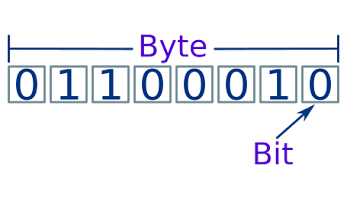
\includegraphics[width=4cm]{images/byte.png}
\centering
\caption{8 bit's (recipientes)  agrupados en bloques de 8 llamados byte. fuente imagen https://terminosaudiovisuales.es/byte/}
\label{fig:byte}
\end{figure}
\[2^{8}=256 \]
De manera abstracta podemos pensar en que cada número entre los 256 que se pueden obtener tras convinar los dos estados, pueden representar  análogamente una letra, número o simbolo de nuestro alfabeto , y qué la disposición de millones de bloques de nuestros recipientes pueden almacenar muchísimas representaciones abstractas de nuestro vocabulario y más.
Inmediatamente nos surge una pregunta qué a veces puede parecer casí que sub-real y es ¿cómo podemos incrustar millónes de estos componentes en una pláca que tiene un tamaño similar a su dedo indice?. Si bien no profundizaré en las técnicas de grabado de estos circuitos si podemos formular una idea más puntual sobre que es la memoria , en sintesis nos permite almacenár la información que será procesada por el microcontrolador del computador, dada sus carácteristicas físicas permite algunas mejoras sutanciales  respecto a la velocidad de acceso y notorias ventajas como un sítio donde se puede almacenar / eliminar / mover y cambiar la información que será dispuesta por el procesador.

\section{Tipos de memoria}

Esta sección es para ver qué pasa con los comandos 
que definen texto

\section{Gestión de la memoria}
A continuación se presenta el logo de C++ Figura 

\section{Comparativa entre memorias}
 esta es la comparativa de las memorias

\section{Conclusión} 
conclusión del documento



\bibliographystyle{IEEEtran}
\bibliography{references}
\cite{rebollo}
\cite{figura1}
\end{document}
